\documentclass[conference]{IEEEtran}
\IEEEoverridecommandlockouts
% Official IEEE conference template (IEEEtran.cls v1.8b, conference_101719.tex layout).
% Every number in this file is generated by ../scripts/a10_paper_assets.py from the per-image
% predictions in github.com/AnshulSinghhhhhh/vision (results/raw). Nothing was re-run on a GPU.
% Items marked [PROPOSED] are experiments that have NOT been run.
\usepackage{cite}
\usepackage{amsmath,amssymb,amsfonts}
\usepackage{graphicx}
\usepackage{textcomp}
\usepackage{xcolor}
\usepackage{booktabs}
\usepackage{url}
\newcommand{\pp}{\,\mathrm{pp}}
\newcommand{\proposed}{\textbf{[PROPOSED]}}
\def\BibTeX{{\rm B\kern-.05em{\sc i\kern-.025em b}\kern-.08em
    T\kern-.1667em\lower.7ex\hbox{E}\kern-.125emX}}
\begin{document}

\title{Spectral Pass-Through or Grid Mismatch? Decomposing Why Higher Test Resolution Amplifies Corruption Damage in CNNs and Vision Transformers}

\author{\IEEEauthorblockN{[Author 1]}
\IEEEauthorblockA{\textit{[Department]} \\
\textit{[Institution]}\\
[City, Country] \\
[email]}
\and
\IEEEauthorblockN{[Author 2]}
\IEEEauthorblockA{\textit{[Department]} \\
\textit{[Institution]}\\
[City, Country] \\
[email]}
}

\maketitle

\begin{abstract}
Running a pretrained classifier at a higher test resolution usually buys clean accuracy, but when the image is corrupted at capture the extra pixels can cost far more than they return. We study this interaction with fixed ImageNet-1k checkpoints by injecting corruptions into a 448-pixel acquisition frame and evaluating the same weights at 224--448 pixels on up to 50,000 paired images. Under Gaussian noise the paired difference-in-differences between 448 and 224 pixels is $-21.9\pp$ for EfficientNet-B3, $-7.2\pp$ for FlexiViT-B and $-4.1\pp$ for DeiT-B/16 (all $|z|>22$). We introduce an exact per-image decomposition that adds an information-matched control, the 224-pixel image upsampled back to 448 pixels, and splits the interaction into a spectral pass-through term (frequencies the anti-aliasing filter would have removed) and a grid term (the same information processed on a finer grid). The terms dissociate by architecture: at the highest noise severity the spectral term carries 89\% of EfficientNet-B3's $-58.7\pp$ penalty but only 13\% of DeiT-B's $-20.5\pp$, while FlexiViT run at a constant 256-token grid has no grid term ($+0.6\pm1.2\pp$). Band-limited noise localizes the damage: the CNN loses most to high-band noise, the vision transformers to mid-band noise ($-47.3\pp$ for DeiT). Consistent with the decomposition, low-pass prefiltering at 448 pixels restores the CNN but not DeiT, whereas a coarser token grid restores FlexiViT. All results are recomputed from released per-image predictions.
\end{abstract}

\begin{IEEEkeywords}
robustness, common corruptions, input resolution, vision transformers, convolutional neural networks, anti-aliasing
\end{IEEEkeywords}

\section{Introduction}
Input resolution is one of the cheapest knobs available at inference time. Evaluating a network at a higher test resolution than it was trained at often improves clean accuracy~\cite{touvron2019fixres}, and flexible architectures make the knob explicit~\cite{beyer2023flexivit,tian2023resformer,dehghani2023navit}. Deployed cameras, however, deliver noisy, blurred and compressed frames~\cite{dodge2016quality,hendrycks2019benchmarking}. If a corruption is fixed at capture, what does spending more pixels on it buy?

Part of the answer is known. Across 1,174 pretrained models, checkpoints with smaller input resolution are more robust to Gaussian noise, and anti-aliased downsampling provably attenuates i.i.d.\ noise~\cite{kim2025noise}. That argument predicts a penalty for higher resolution, but it compares different checkpoints, and a single model run at a higher resolution changes two things at once. First, \emph{spectral pass-through}: frequencies above the lower resolution's Nyquist limit, which the anti-aliasing filter would have removed, now reach the network. Second, \emph{grid mismatch}: the same content is rendered on a finer pixel grid, so objects look larger, and for vision transformers (ViTs) the token count grows and position embeddings are interpolated. Both effects grow with resolution, so a plain resolution sweep cannot tell them apart. Which one dominates determines the remedy: a low-pass filter fixes the first but not the second.

We separate the two effects with an information-matched control. The corrupted acquisition frame is rendered (A) at 448 pixels, (C) downsampled to 224 pixels, and (D) downsampled to 224 and upsampled back to 448 pixels. Rendering D carries exactly the information of C on the grid of A, so the per-image identity $\mathrm{A}-\mathrm{C}=(\mathrm{A}-\mathrm{D})+(\mathrm{D}-\mathrm{C})$ splits the resolution effect into a spectral and a grid term with no modeling assumptions.

\textbf{Contributions.} (i) A paired difference-in-differences protocol with corruptions fixed in an acquisition frame, applied to three architectures, four corruptions and three severities on up to 50,000 ImageNet validation images. (ii) An exact spectral/grid decomposition showing that the two mechanisms dissociate by architecture: the penalty is about 90\% spectral for EfficientNet-B3 but almost entirely grid-driven for DeiT-B/16. (iii) Frequency localization with band-limited noise: the CNN is hurt by high-band noise, the ViTs by mid-band noise. (iv) Prescriptive consequences confirmed by independent controls: input low-pass filtering repairs the CNN but not DeiT, while a coarser token grid repairs FlexiViT.

\section{Related Work}
\textbf{Corruption robustness and frequency.} ImageNet-C~\cite{hendrycks2019benchmarking} standardized synthetic corruptions at 224 pixels; earlier work measured how noise, blur and compression degrade classifiers~\cite{dodge2016quality}. Fourier analyses show that naturally trained CNNs are sensitive to high-frequency perturbations~\cite{yin2019fourier}, whereas self-attention acts as a low-pass filter, making ViTs comparatively robust to high-frequency but vulnerable to low-frequency noise~\cite{park2022how,shao2022adversarial,kim2024spectral}. These studies fix the resolution; we ask how changing it moves a fixed corruption relative to each architecture's sensitivity.

\textbf{Resolution and anti-aliasing.} FixRes~\cite{touvron2019fixres} attributes test-resolution gains to the apparent object size mismatch between training and testing crops. Anti-aliasing improves shift invariance and robustness of CNNs~\cite{zhang2019shift,vasconcelos2021aliasing}. Kim~et~al.~\cite{kim2025noise} relate smaller input resolution, larger stem kernels and larger patches to noise robustness across checkpoints and bound the noise gain of anti-aliased downsampling. Our study is complementary: within one set of weights, we measure how much of the resolution penalty is that noise gain and how much is not.

\textbf{Resolution-flexible ViTs and token budgets.} FlexiViT trains one model for many patch sizes~\cite{beyer2023flexivit}; ResFormer, NaViT and ViTAR target resolution generalization~\cite{tian2023resformer,dehghani2023navit,fan2024vitar}. Token reduction~\cite{bolya2023tome} degrades under distribution shift unless reductions are scheduled late~\cite{cha2026later}. We use FlexiViT's patch size as a controlled way to change the token grid at a fixed input.

\section{Methodology}
\subsection{Acquisition model and resampling}
Each validation image is resized (short side 512) and center-cropped to an acquisition frame $x_i\in[0,1]^{448\times448\times3}$. A corruption $c$ of severity $s$ is applied once, with a seed $\xi_i$ derived from $(\text{image},c,s)$ by SHA-256:
\begin{equation}
\tilde x_i = c_s(x_i;\xi_i).
\end{equation}
The network at resolution $R$ receives $S_R\tilde x_i$, where $S_R$ is separable anti-aliased bilinear resampling. Its 1-D weights for output sample $m$ are a triangle stretched by the scale factor $\rho=448/R$,
\begin{equation}
w_{m,k}\propto\max\!\Big(0,\,1-\tfrac{|k-\mu_m|}{\rho}\Big),\quad \mu_m=\big(m+\tfrac12\big)\rho-\tfrac12,
\end{equation}
normalized to unit sum. For i.i.d.\ noise of standard deviation $\sigma$, the output standard deviation is $g_R\sigma$ with
\begin{equation}
g_R=\frac{1}{R}\sum_{m}\sum_{k}w_{m,k}^2 ,
\end{equation}
giving $g_R=0.313,0.481,0.566,1.000$ for $R=224,320,384,448$ (measured on white noise: 0.313, 0.481, 0.566). At 448 pixels the resampler is the identity, so the network sees about $1/g_{224}^2\approx10\times$ more noise variance than at 224 pixels.

\subsection{Paired interaction statistic}
Let $y_i(R,s)\in\{0,1\}$ indicate a correct top-1 prediction, with $s=0$ denoting the clean image. The per-image interaction between resolution and corruption is
\begin{equation}
D_i=\big[y_i(448,s)-y_i(224,s)\big]-\big[y_i(448,0)-y_i(224,0)\big],\label{eq:did}
\end{equation}
and the difference-in-differences (DiD) is $\Delta=\frac1N\sum_iD_i$, reported in percentage points. Because all four cells are observed on the same images,
\begin{equation}
\widehat{\mathrm{SE}}(\Delta)=\frac{\hat\sigma_D}{\sqrt N},\qquad z=\frac{\Delta}{\widehat{\mathrm{SE}}(\Delta)},\label{eq:se}
\end{equation}
with Holm's step-down correction~\cite{holm1979} across the twelve primary (model, corruption) tests. A negative $\Delta$ means that the higher resolution helps less, or hurts more, under corruption than on clean images.

\subsection{Spectral/grid decomposition}
For each corrupted frame we form four renderings and evaluate the same weights on each:
\begin{align}
\mathrm{A}&=\tilde x, & \mathrm{C}&=S_{224}\tilde x,\nonumber\\
\mathrm{D}&=U\,S_{224}\tilde x, & \mathrm{B}&=h\ast\tilde x,
\end{align}
where $U$ is $2\times$ bilinear upsampling and $h$ the 3-tap binomial kernel $[\tfrac14,\tfrac12,\tfrac14]^{\otimes2}$ applied without decimation. Writing $\Delta(\mathrm{P},\mathrm{Q})$ for the DiD of \eqref{eq:did} with renderings P and Q in place of 448 and 224 pixels, the per-image identity
\begin{equation}
\underbrace{\Delta(\mathrm{A},\mathrm{C})}_{\Delta}=\underbrace{\Delta(\mathrm{A},\mathrm{D})}_{\Delta_{\mathrm{spec}}}+\underbrace{\Delta(\mathrm{D},\mathrm{C})}_{\Delta_{\mathrm{grid}}}\label{eq:decomp}
\end{equation}
holds exactly. D contains no more information than C and lives on the grid of A. $\Delta_{\mathrm{grid}}$ is therefore the cost of processing a fixed, band-limited content on the finer grid. $\Delta_{\mathrm{spec}}$ is the cost of the content that the 224-pixel path discards, mainly frequencies above its Nyquist limit. We report the spectral share $\varphi=\Delta_{\mathrm{spec}}/\Delta$ when $|\Delta|$ is large. Because C is a deterministic function of A, a Bayes-optimal classifier on A can never be less accurate than on C, so a negative $\Delta$ is a property of the learned weights, not lost information.

\subsection{Band-limited noise}
To localize the effect in frequency, white Gaussian fields $w$ are masked in the Fourier domain by annuli $M_b$ (radii in cycles per 448-pixel frame) and rescaled to a target pre-clipping RMS $r_s$:
\begin{equation}
n_b=\kappa\,\mathcal F^{-1}\!\left[M_b\odot\mathcal F[w]\right],\qquad \tilde x=\mathrm{clip}(x+n_b),
\end{equation}
with bands low $[0,56)$, mid $[56,112)$, high $[112,224]$ and broadband, and $r_3=45.9$, $r_5=96.9$ on a 0--255 scale (matching the Gaussian-noise $\sigma$ of severities 3 and 5). The 224-pixel Nyquist frequency is 112 cycles per frame, so the high band lies entirely above it. Post-clipping RMS is equal across bands (41.55 and 75.25).

\section{Experimental Setup}
\textbf{Models.} DeiT-B/16 (\texttt{deit\_base\_patch16\_224.fb\_in1k})~\cite{touvron2021deit} with interpolated position embeddings; EfficientNet-B3 (\texttt{efficientnet\_b3.ra2\_in1k}, native test resolution 320)~\cite{tan2019efficientnet}; FlexiViT-B (\texttt{flexivit\_base.1200ep\_in1k})~\cite{beyer2023flexivit} in two arms, \emph{F-p} (patch 16, 196--784 tokens) and \emph{F-t} (a fixed $16\times16$ grid, patch $R/16$); for replication, ResNet-50 (\texttt{a1\_in1k})~\cite{wightman2021resnet} and ConvNeXt-B (\texttt{fb\_in22k\_ft\_in1k})~\cite{liu2022convnext}, all from timm~\cite{wightman2019timm}. With their native preprocessing, the four primary checkpoints (including DeiT-B/16-384) reproduce their published top-1 accuracy within 0.21\,pp on the full 50,000-image validation set~\cite{russakovsky2015imagenet}.

\textbf{Corruptions.} Gaussian noise ($\sigma=0.08,0.18,0.38$ for severities 1, 3, 5), defocus blur (ImageNet-C disk kernel), JPEG (quality 15) and contrast (factor 0.2) at severity 3, following~\cite{hendrycks2019benchmarking} but applied in the 448-pixel frame.

\textbf{Samples.} Headline cells use all 50,000 validation images (clean and severity 3) or 15,000 class-balanced images (severities 1 and 5). The decomposition (A/B/C/D) uses 2,000 class-balanced images; the B-filter replication uses 10,000 images (three models) and 5,000 (ResNet-50, ConvNeXt-B); band-limited noise 2,000; resize operators 5,000; the FlexiViT patch grid 3,000.

\textbf{Provenance and reliability.} Inference ran in fp16 autocast on NVIDIA T4 GPUs; fp16 and fp32 gave identical accuracy on a 500-image check. Separately executed experiments produced identical per-image predictions on shared (image, configuration) pairs in at least 99.7\% of cases for clean and noisy inputs. In the headline run the defocus corruption was a Gaussian-blur stand-in rather than the ImageNet-C disk kernel (86--95\% per-image agreement), so we report defocus only from the 10,000-image run with the verified kernel. Statistics are paired as in \eqref{eq:did}--\eqref{eq:se}. A re-analysis restricted to the 44,000 images held out from all pilot decisions, and a log-odds version of every DiD (image bootstrap, 1,000 resamples), leave all signs and conclusions unchanged.

\section{Results}
\subsection{Higher resolution amplifies corruption damage}
Table~\ref{tab:did} and Fig.~\ref{fig:curves} summarize the interaction. Under Gaussian noise the DiD is negative for all three models and grows super-linearly with severity. For EfficientNet-B3, $-1.6\pp$ at severity 1 becomes $-59.9\pp$ at severity 5, where accuracy at 448 pixels falls to 3.7\%. The collapse is not an artefact of EfficientNet's sub-native 224 baseline: measured from its native 320 pixels, the severity-3 DiD is still $-21.5\pm0.4\pp$. The models disagree on the other corruptions. DeiT-B loses at 448 pixels under every corruption, including contrast ($-1.27\pp$). EfficientNet-B3 gains under contrast from 224 pixels ($+1.16\pp$), but this gain vanishes from its native resolution (320$\to$448: $-0.00\pm0.22\pp$). With the verified defocus kernel, FlexiViT shows no interaction ($-0.24\pm0.60\pp$), whereas DeiT loses $6.04\pm0.84\pp$.

\begin{table}[t]
\caption{Resolution$\times$corruption DiD (pp), 448 vs.\ 224 pixels, with 95\% CI half-widths. $N=50{,}000$ unless noted; $\dagger$: $N=15{,}000$ (secondary); $\ddagger$: ImageNet-C disk defocus, $N=10{,}000$. Severity-3 noise, JPEG and contrast rows: Holm-adjusted $p<0.002$ over the primary tests; FlexiViT defocus is not significant.}
\label{tab:did}
\centering
\setlength{\tabcolsep}{4pt}
\begin{tabular}{lccc}
\toprule
 & EffNet-B3 & FlexiViT-B (F-p) & DeiT-B/16\\
\midrule
Clean gain $\Delta_{448-224}$ & $+4.42$ & $+0.72$ & $-1.60$\\
Noise s1$^\dagger$ & $-1.64\pm0.56$ & $-1.91\pm0.45$ & $-0.77\pm0.54$\\
Noise s3 & $-21.92\pm0.48$ & $-7.21\pm0.34$ & $-4.08\pm0.36$\\
Noise s5$^\dagger$ & $-59.85\pm0.90$ & $-43.72\pm0.89$ & $-19.71\pm0.85$\\
Defocus s3$^\ddagger$ & $-1.71\pm0.87$ & $-0.24\pm0.60$ & $-6.04\pm0.84$\\
JPEG s3 & $-0.60\pm0.33$ & $-2.45\pm0.27$ & $-5.41\pm0.36$\\
Contrast s3 & $+1.16\pm0.27$ & $+0.70\pm0.22$ & $-1.27\pm0.29$\\
\bottomrule
\end{tabular}
\end{table}

\begin{figure}[t]
\centering
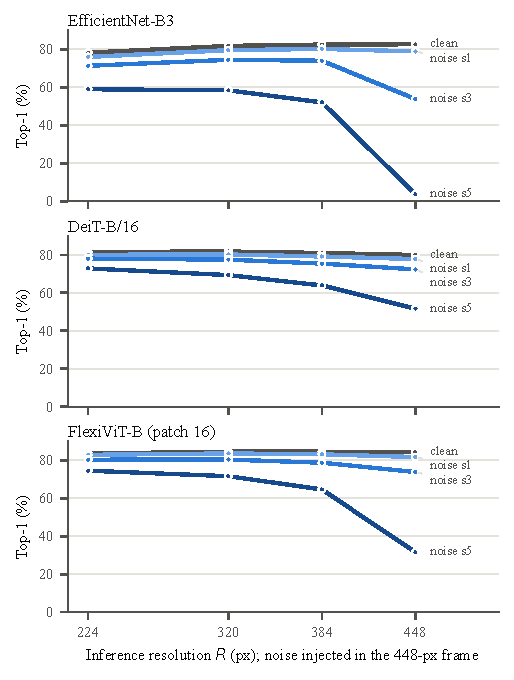
\includegraphics[width=\columnwidth]{figures/fig1_resolution_curves.pdf}
\caption{Top-1 accuracy of the same weights at four test resolutions; noise is injected once in the 448-pixel frame and the frame is resampled with anti-aliasing. $N=50{,}000$ (clean, s3) and $15{,}000$ (s1, s5).}
\label{fig:curves}
\end{figure}

\subsection{The penalty has two mechanisms that dissociate by architecture}
Table~\ref{tab:decomp} and Fig.~\ref{fig:decomp} apply the decomposition \eqref{eq:decomp}. For EfficientNet-B3 the spectral term carries almost the whole noise penalty ($\varphi=0.93$ at s3, $0.89$ at s5): once the frequencies above the 224-pixel Nyquist limit are removed, the 448-pixel grid costs only $-1.45\pp$ (s3). DeiT-B behaves in the opposite way. Re-presenting the 224-pixel information on the 448-pixel grid already costs $-17.85\pm2.39\pp$ at s5 ($\varphi=0.13$). At s3 the extra high-frequency content actually helps DeiT ($\Delta_{\mathrm{spec}}=+3.75\pm1.94\pp$) while the grid term is $-7.50\pm1.98\pp$. FlexiViT with a fixed patch size (F-p) is mixed ($\varphi=0.72$--$0.79$). The same weights run at a constant 256-token grid (F-t) show no grid term at any severity ($+0.55\pm1.16\pp$ at s5), and the remaining spectral term is small ($-7.60\pp$). Under verified defocus blur the high frequencies help every model ($\Delta_{\mathrm{spec}}\ge+0.70\pp$), and whatever penalty remains is a grid effect, largest for DeiT ($-8.10\pm2.08\pp$).

\begin{table}[t]
\caption{Exact decomposition $\Delta=\Delta_{\mathrm{spec}}+\Delta_{\mathrm{grid}}$ (pp, 95\% CI half-widths), $N=2{,}000$ paired images. Defocus uses the ImageNet-C disk kernel.}
\label{tab:decomp}
\centering
\setlength{\tabcolsep}{3.2pt}
\begin{tabular}{llccc}
\toprule
Model & Corruption & $\Delta$ & $\Delta_{\mathrm{spec}}$ (A$-$D) & $\Delta_{\mathrm{grid}}$ (D$-$C)\\
\midrule
EffNet-B3 & noise s3 & $-21.80\pm2.41$ & $-20.35\pm2.27$ & $-1.45\pm1.84$\\
 & noise s5 & $-58.70\pm2.49$ & $-52.30\pm2.43$ & $-6.40\pm2.21$\\
 & defocus s3 & $-2.70\pm2.12$ & $+2.15\pm1.49$ & $-4.85\pm2.10$\\
\midrule
FlexiViT F-p & noise s3 & $-7.50\pm1.72$ & $-5.40\pm1.57$ & $-2.10\pm1.43$\\
 & noise s5 & $-42.70\pm2.41$ & $-33.65\pm2.33$ & $-9.05\pm1.82$\\
 & defocus s3 & $-0.70\pm1.39$ & $+1.35\pm1.33$ & $-2.05\pm1.41$\\
\midrule
FlexiViT F-t & noise s3 & $-1.50\pm1.22$ & $-1.30\pm1.35$ & $-0.20\pm0.96$\\
 & noise s5 & $-7.05\pm1.65$ & $-7.60\pm1.80$ & $+0.55\pm1.16$\\
 & defocus s3 & $+0.50\pm1.02$ & $+0.70\pm1.35$ & $-0.20\pm0.98$\\
\midrule
DeiT-B/16 & noise s3 & $-3.75\pm1.88$ & $+3.75\pm1.94$ & $-7.50\pm1.98$\\
 & noise s5 & $-20.50\pm2.33$ & $-2.65\pm2.20$ & $-17.85\pm2.39$\\
 & defocus s3 & $-6.75\pm1.96$ & $+1.35\pm1.59$ & $-8.10\pm2.08$\\
\bottomrule
\end{tabular}
\end{table}

\begin{figure}[t]
\centering
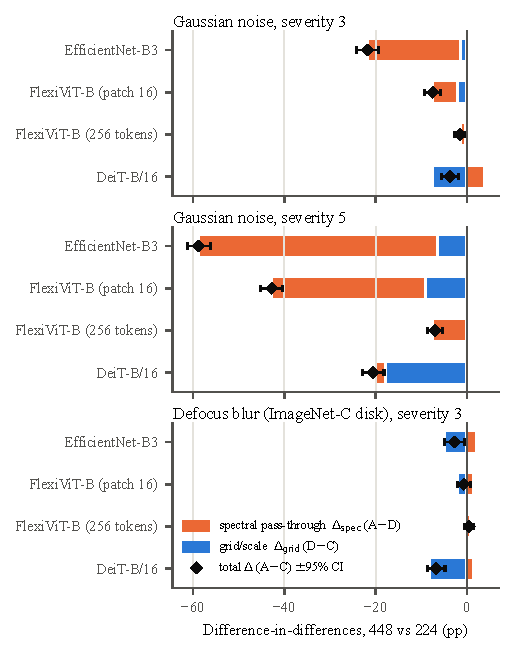
\includegraphics[width=\columnwidth]{figures/fig2_decomposition.pdf}
\caption{Spectral (orange) and grid (blue) terms of the 448-vs-224 interaction. Diamonds: total $\Delta$ with 95\% CI. EfficientNet's penalty is spectral; DeiT's is grid-driven; FlexiViT at a fixed token grid has no grid term.}
\label{fig:decomp}
\end{figure}

\subsection{Replication with low-pass filters at 448 pixels}
The 3-tap filter B removes most, but not all, of the content above the 224-pixel Nyquist limit while keeping the 448-pixel grid. On 10,000 images (Table~\ref{tab:bfilter}), B removes 93\% (s3) and 85\% (s5) of EfficientNet's penalty, 38\% and 67\% of FlexiViT-p's, and 22\% of DeiT's at s5. At s3, B makes DeiT \emph{worse} ($-6.44$ vs.\ $-4.90\pp$). A Gaussian prefilter ($\sigma=0.866$\,px, 5,000 images) tells the same story. At s5 it lifts EfficientNet at 448 pixels by $+51.3\pm1.4\pp$ to within $4.6\pm1.2\pp$ of the 224-pixel baseline, but lifts DeiT by only $+4.2\pm1.1\pp$, leaving it $17.2\pm1.2\pp$ below 224 pixels. At s3 the prefilter lowers DeiT's accuracy ($-2.5\pm0.9\pp$). Across a sweep of Gaussian widths (0.5--2.5\,px), no prefilter brings DeiT within 16\,pp of its 224-pixel accuracy at s5. Two further CNNs fall between the extremes: B removes 71\% of ConvNeXt-B's s5 penalty but only 33\% of ResNet-50's. Without a D control for these models the residual cannot be attributed (Section~\ref{sec:limits}).

\begin{table}[t]
\caption{3-tap low-pass at 448 pixels (B): total DiD $\Delta$ (A vs.\ C), residual $\Delta(\mathrm{B},\mathrm{C})$, and share removed, Gaussian noise s5 (s3 in brackets). 95\% CI half-widths $\le1.1\pp$ ($N=10{,}000$) and $\le1.7\pp$ ($N=5{,}000$).}
\label{tab:bfilter}
\centering
\setlength{\tabcolsep}{3.5pt}
\begin{tabular}{lrrr}
\toprule
Model ($N$) & $\Delta$ & residual & removed\\
\midrule
EffNet-B3 (10k) & $-58.95$\,[$-22.18$] & $-8.89$\,[$-1.57$] & 85\%\,[93\%]\\
FlexiViT F-p (10k) & $-43.22$\,[$-7.26$] & $-14.37$\,[$-4.51$] & 67\%\,[38\%]\\
DeiT-B/16 (10k) & $-19.54$\,[$-4.90$] & $-15.24$\,[$-6.44$] & 22\%\,[$-31$\%]\\
ConvNeXt-B (5k) & $-35.84$\,[$-2.94$] & $-10.22$\,[$-3.18$] & 71\%\,[$-8$\%]\\
ResNet-50 (5k) & $-40.40$\,[$-20.90$] & $-26.98$\,[$-10.14$] & 33\%\,[51\%]\\
\bottomrule
\end{tabular}
\end{table}

\subsection{Where in frequency the damage occurs}
Band-limited noise (Fig.~\ref{fig:bands}) shows the same split. For EfficientNet the largest interaction comes from the high band, which the 224-pixel path removes ($-54.95\pm2.51\pp$ at s5), and low-band noise leaves its accuracy flat across resolutions (40.5\% at 224 vs.\ 40.3\% at 448 pixels, s3). For both ViTs the largest interaction comes from the mid band: DeiT $-47.35\pm2.59\pp$ and FlexiViT-p $-73.60\pm2.14\pp$ at s5, compared with $-13.05$ and $-37.00\pp$ for the high band. Unlike EfficientNet, DeiT also loses to low-band noise as resolution grows (53.6\% $\to$ 38.3\% at s3), even though anti-aliasing barely attenuates that band. At 448 pixels a mid-band period of 4--8 pixels corresponds to 2--4 cycles per 16-pixel patch. We hypothesize that this places the noise in the passband of the patch embedding. With the token grid fixed (F-t), the mid-band interaction shrinks from $-41.15$ to $-5.95\pp$ at s3, but not at s5 ($-53.85\pp$).

\begin{figure}[t]
\centering
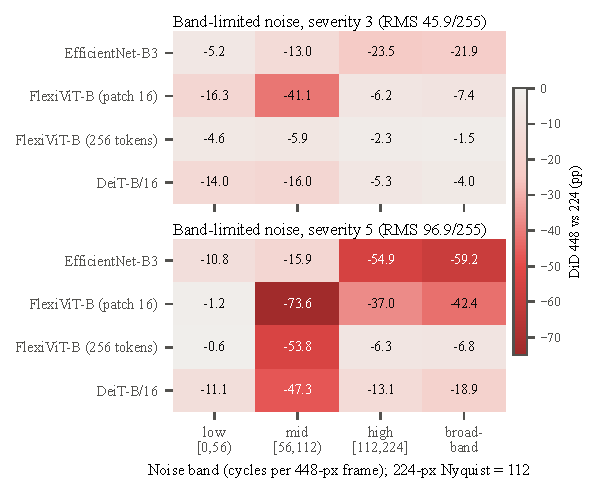
\includegraphics[width=\columnwidth]{figures/fig3_band_did.pdf}
\caption{DiD (448 vs.\ 224 pixels, pp) for noise confined to Fourier annuli, at equal pre-clipping RMS; $N=2{,}000$ per arm; SE 0.4--1.3\,pp. The CNN is hurt most by the band above the 224-pixel Nyquist limit, the ViTs by the mid band.}
\label{fig:bands}
\end{figure}

\subsection{Noise gain explains the CNN, not the ViT}
Fig.~\ref{fig:gain} plots accuracy against the measured white-noise gain of six resize operators at three resolutions. For EfficientNet, accuracy at severity 5 follows the gain closely (Spearman $\rho=-0.92$, $p=4\times10^{-6}$, 14 operator--resolution cells). Area averaging and non-anti-aliased bilinear resizing at 224 pixels both reduce to a $2\times2$ box (gain 0.500) and produce identical predictions. EfficientNet's 20-point deficit for these operators relative to anti-aliased bilinear resizing therefore reflects noise gain, not aliasing. For DeiT the rank correlation is weak ($-0.41$, $p=0.14$): resolution, not gain, orders its accuracy. The prefiltered 448-pixel input has nearly the lowest gain (0.327) yet sits near the bottom of the plot.

\begin{figure}[t]
\centering
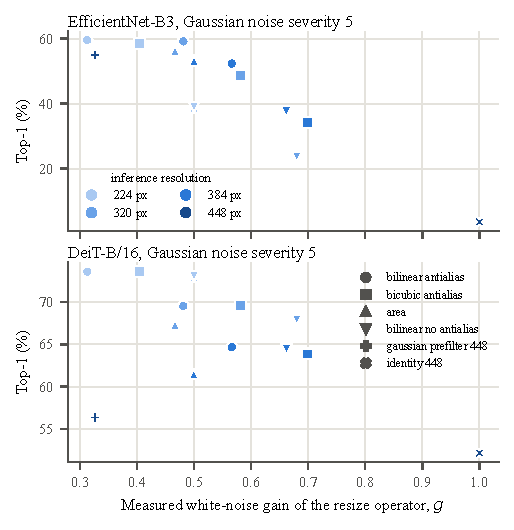
\includegraphics[width=\columnwidth]{figures/fig4_operator_gain.pdf}
\caption{Accuracy under severity-5 noise against the measured noise gain of the resize operator (marker: operator; shade: resolution); $N=5{,}000$. Area and non-anti-aliased bilinear at 224 pixels coincide.}
\label{fig:gain}
\end{figure}

\subsection{Removing the grid term with a coarser token grid}
If the ViT penalty is a grid effect, changing the token grid at a fixed input should recover it. With FlexiViT at 448 pixels ($N=3{,}000$), switching from 16- to 32-pixel patches (784 to 196 tokens) raises severity-5 accuracy from 30.97\% to 70.10\% ($+39.13\pm1.82\pp$) and severity-3 accuracy by $+6.67\pm1.14\pp$, at no clean cost ($-0.37\pm0.69\pp$). Compared with 16-pixel patches on the 224-pixel image (also 196 tokens), the 448/32 configuration is better on clean ($+0.63\pm0.78\pp$) and defocused inputs ($+1.63\pm0.71\pp$), equal at s3 ($-0.37\pm0.74\pp$) and worse at s5 ($-4.67\pm1.14\pp$). A larger patch with resampled embedding weights also low-pass filters inside the embedding, so this experiment cannot separate token count from that implicit filter. It does show that for a flexible ViT the remedy can stay inside the model.

\subsection{The grid term is not a confidence-margin artefact}
One might expect DeiT to lose more under corruption at 448 pixels simply because its predictions are less confident there. They are not: among correctly classified clean images, its mean max-softmax confidence is 0.806 at 448 pixels and 0.796 at 224. Standardizing for clean confidence (ten bins) on the roughly 40,000 clean-correct images per cell, DeiT's corruption-induced flip rate at 448 pixels still exceeds the rate expected at 224 pixels by $+6.1\pp$ (noise), $+7.7\pp$ (JPEG) and $+2.0\pp$ (contrast); FlexiViT-p shows $+9.9\pp$ for noise. EfficientNet's confidence calibration shifts with resolution (0.816$\to$0.641), so this control is not informative for it.

\section{Discussion}
\textbf{Two failure modes, two remedies.} A resolution increase hurts a corrupted image for different reasons in different architectures. For the CNN studied here the loss is overwhelmingly the noise that downsampling would have averaged away~\cite{kim2025noise}; band-limiting the input at the higher resolution, or simply downsampling, restores it. For the fixed-patch ViT the input spectrum is almost irrelevant: the same information on a finer grid is processed less robustly, and filtering does not help. For a flexible-patch ViT the grid term disappears when the token grid is held fixed. In practice, the safe default for noisy captures is to downsample to the model's native token grid. Prefiltering at high resolution is only a remedy when the model's penalty is spectral.

\textbf{Why DeiT has a grid term.} At 448 pixels DeiT interpolates position embeddings from a $14\times14$ to a $28\times28$ grid, sees objects at twice their training scale and attends over four times as many tokens. Its native-384 checkpoint is $6.35\pm0.63\pp$ more accurate than the interpolated 224 checkpoint at 384 pixels under severity-5 noise (15,000 images), compared with $+1.20\pm0.82\pp$ on clean images. Resolution-specific fine-tuning therefore shrinks the problem but does not remove it. The existing data cannot apportion the grid term among position embeddings, scale and token count.

\textbf{Relation to frequency biases.} ViTs are known to be vulnerable to lower-frequency noise than CNNs~\cite{park2022how}. Our band results add a resolution axis to that picture: raising the resolution stretches a fixed physical noise band to longer pixel periods, moving mid-band noise to 2--4 cycles per patch, where the ViTs studied here are most sensitive.

\section{Limitations}
\label{sec:limits}
(1) One checkpoint per family; the decomposition covers three architectures (four configurations), on 2,000 images. (2) The 448-pixel frame is produced by resizing the short side to 512 pixels. Many ImageNet validation images have a shorter short side, so the frame is often an upsampled image, and noise is added after that upsampling rather than at a sensor grid. Native image sizes were not recorded, so we cannot quantify this or stratify by it. (3) Corruptions are synthetic and drawn once per image, so CIs reflect image sampling only. (4) B is a 3-tap filter, not an exact information match; only D is. ResNet-50 and ConvNeXt-B lack D. (5) Only ImageNet-1k classification is studied.

\textbf{Remaining experiments.} \proposed~E1: the D control at $N=10{,}000$ for ResNet-50, ConvNeXt-B, a hierarchical ViT, a ViT with absolute and one with rotary position embeddings, and for JPEG and contrast (about 0.5--1 T4 GPU-hour per model). \proposed~E2: three noise draws per image. \proposed~E3: stratification by native image size from JPEG headers (CPU only). \proposed~E4: band-limited noise combined with D. \proposed~E5: the decomposition at 320 and 384 pixels. \proposed~E6: Poisson--Gaussian noise injected at the native sensor grid. \proposed~E7: D built with nearest, bicubic and Lanczos upsamplers, to rule out that the grid term reflects the smoothness of bilinear upsampling (D is $1.95\pp$ below A for DeiT on clean images, a difference the DiD removes only to first order).

\section{Conclusion}
When a corruption is fixed at capture, raising the test resolution of a pretrained classifier amplifies its damage, but not for one reason. An exact decomposition built on an information-matched upsample-back control shows that the penalty is spectral pass-through for EfficientNet-B3 and grid mismatch for DeiT-B/16, with FlexiViT in between unless its token grid is held fixed. The mechanism determines the fix: low-pass filtering for the former, the native token grid for the latter.

\section*{Acknowledgment}
[Funding and acknowledgments.] \emph{AI disclosure (adapt to the venue's policy):} the experiment code in the source repository was written with the assistance of an AI coding agent. The audit, statistical re-analysis, figures and text of this manuscript were drafted with Claude (Anthropic) from the released per-image predictions. The authors checked every reported number against the raw data.

\begin{thebibliography}{00}
\bibitem{touvron2019fixres} H. Touvron, A. Vedaldi, M. Douze, and H. J\'egou, ``Fixing the train-test resolution discrepancy,'' in \emph{Proc. NeurIPS}, 2019.
\bibitem{beyer2023flexivit} L. Beyer \emph{et al.}, ``FlexiViT: One model for all patch sizes,'' in \emph{Proc. IEEE/CVF CVPR}, 2023.
\bibitem{tian2023resformer} R. Tian \emph{et al.}, ``ResFormer: Scaling ViTs with multi-resolution training,'' in \emph{Proc. IEEE/CVF CVPR}, 2023.
\bibitem{dehghani2023navit} M. Dehghani \emph{et al.}, ``Patch n' Pack: NaViT, a vision transformer for any aspect ratio and resolution,'' in \emph{Proc. NeurIPS}, 2023.
\bibitem{dodge2016quality} S. Dodge and L. Karam, ``Understanding how image quality affects deep neural networks,'' in \emph{Proc. QoMEX}, 2016.
\bibitem{hendrycks2019benchmarking} D. Hendrycks and T. Dietterich, ``Benchmarking neural network robustness to common corruptions and perturbations,'' in \emph{Proc. ICLR}, 2019.
\bibitem{kim2025noise} B. J. Kim, M. Kawano, Y. Iwasawa, and Y. Matsuo, ``Unlocking noise-resistant vision: Key architectural secrets for robust models,'' arXiv:2509.20939, 2025.
\bibitem{yin2019fourier} D. Yin, R. G. Lopes, J. Shlens, E. D. Cubuk, and J. Gilmer, ``A Fourier perspective on model robustness in computer vision,'' in \emph{Proc. NeurIPS}, 2019.
\bibitem{park2022how} N. Park and S. Kim, ``How do vision transformers work?'' in \emph{Proc. ICLR}, 2022.
\bibitem{shao2022adversarial} R. Shao, Z. Shi, J. Yi, P.-Y. Chen, and C.-J. Hsieh, ``On the adversarial robustness of vision transformers,'' \emph{Trans. Mach. Learn. Res.}, 2022.
\bibitem{kim2024spectral} G. Kim \emph{et al.}, ``Exploring adversarial robustness of vision transformers in the spectral perspective,'' in \emph{Proc. IEEE/CVF WACV}, 2024.
\bibitem{zhang2019shift} R. Zhang, ``Making convolutional networks shift-invariant again,'' in \emph{Proc. ICML}, 2019.
\bibitem{vasconcelos2021aliasing} C. Vasconcelos, H. Larochelle, V. Dumoulin, R. Romijnders, N. Le Roux, and R. Goroshin, ``Impact of aliasing on generalization in deep convolutional networks,'' in \emph{Proc. IEEE/CVF ICCV}, 2021.
\bibitem{fan2024vitar} Q. Fan \emph{et al.}, ``ViTAR: Vision transformer with any resolution,'' arXiv:2403.18361, 2024.
\bibitem{bolya2023tome} D. Bolya, C.-Y. Fu, X. Dai, P. Zhang, C. Feichtenhofer, and J. Hoffman, ``Token merging: Your ViT but faster,'' in \emph{Proc. ICLR}, 2023.
\bibitem{cha2026later} H. Cha, H. Yoon, and S.-J. Lee, ``Later is better: Token reduction for ViTs under distribution shift,'' arXiv:2610.07758, 2026.
\bibitem{holm1979} S. Holm, ``A simple sequentially rejective multiple test procedure,'' \emph{Scand. J. Statist.}, vol. 6, no. 2, pp. 65--70, 1979.
\bibitem{touvron2021deit} H. Touvron, M. Cord, M. Douze, F. Massa, A. Sablayrolles, and H. J\'egou, ``Training data-efficient image transformers \& distillation through attention,'' in \emph{Proc. ICML}, 2021.
\bibitem{tan2019efficientnet} M. Tan and Q. V. Le, ``EfficientNet: Rethinking model scaling for convolutional neural networks,'' in \emph{Proc. ICML}, 2019.
\bibitem{wightman2021resnet} R. Wightman, H. Touvron, and H. J\'egou, ``ResNet strikes back: An improved training procedure in timm,'' arXiv:2110.00476, 2021.
\bibitem{liu2022convnext} Z. Liu, H. Mao, C.-Y. Wu, C. Feichtenhofer, T. Darrell, and S. Xie, ``A ConvNet for the 2020s,'' in \emph{Proc. IEEE/CVF CVPR}, 2022.
\bibitem{wightman2019timm} R. Wightman, ``PyTorch image models,'' GitHub repository, 2019. [Online]. Available: \url{https://github.com/huggingface/pytorch-image-models}
\bibitem{russakovsky2015imagenet} O. Russakovsky \emph{et al.}, ``ImageNet large scale visual recognition challenge,'' \emph{Int. J. Comput. Vis.}, vol. 115, no. 3, pp. 211--252, 2015.
\end{thebibliography}

\end{document}
